\section{Diagramme de cas d'utilisation}
	\begin{figure}[!h]
		\centering
		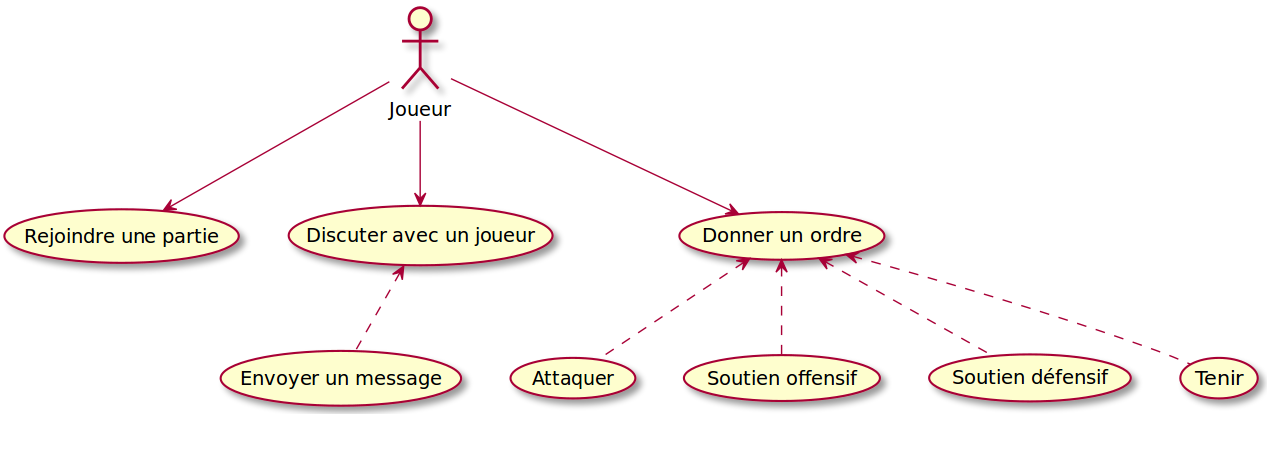
\includegraphics[scale=0.4]{images/UseCase.png}
		\caption{Diagramme de cas d'utilisation}
	\end{figure}
\newpage
\section{Diagramme de classes participantes}
\subsection{Moteur du jeu}
	\begin{figure}[!h]
		\centering
		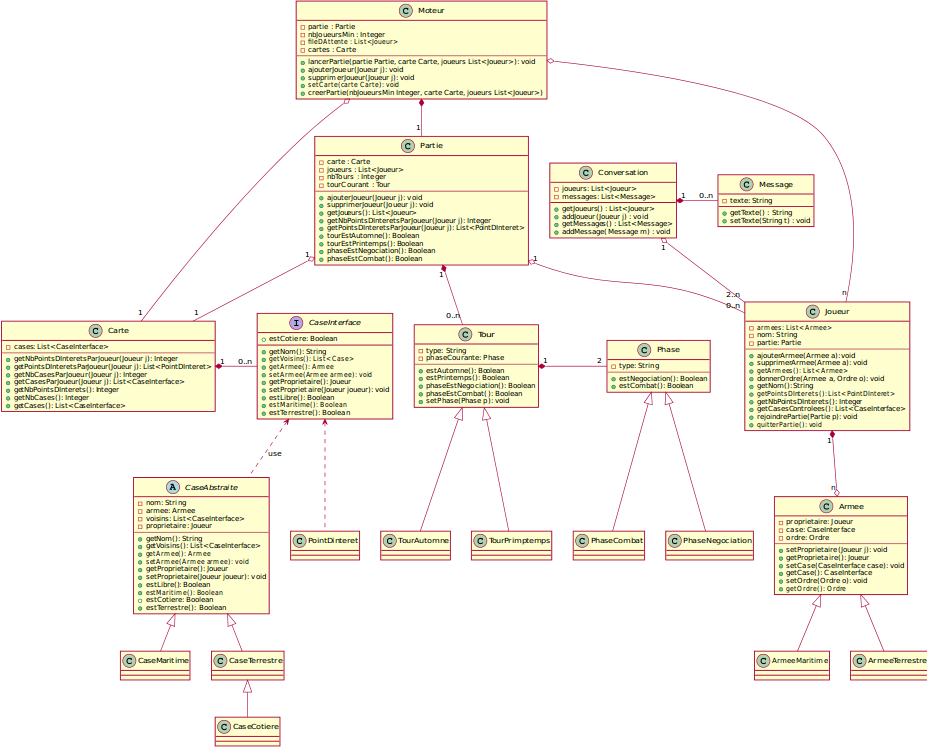
\includegraphics[scale=0.6,angle=90]{images/DCP1.png}
		\caption{Moteur du jeu}
	\end{figure}
\newpage
\subsection{Les ordres}
	\begin{figure}[!h]
		\centering
		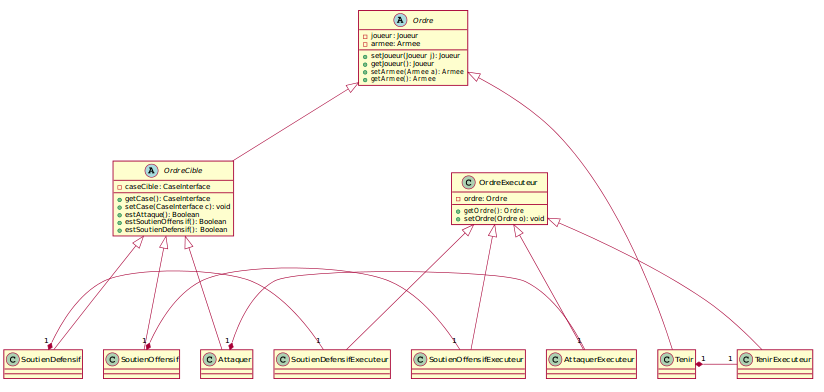
\includegraphics[scale=0.5]{images/DCP2.png}
		\caption{Les ordres}
	\end{figure}

\subsection{Les exceptions}
	\vspace{10mm}
	\begin{figure}[!h]
		\centering
		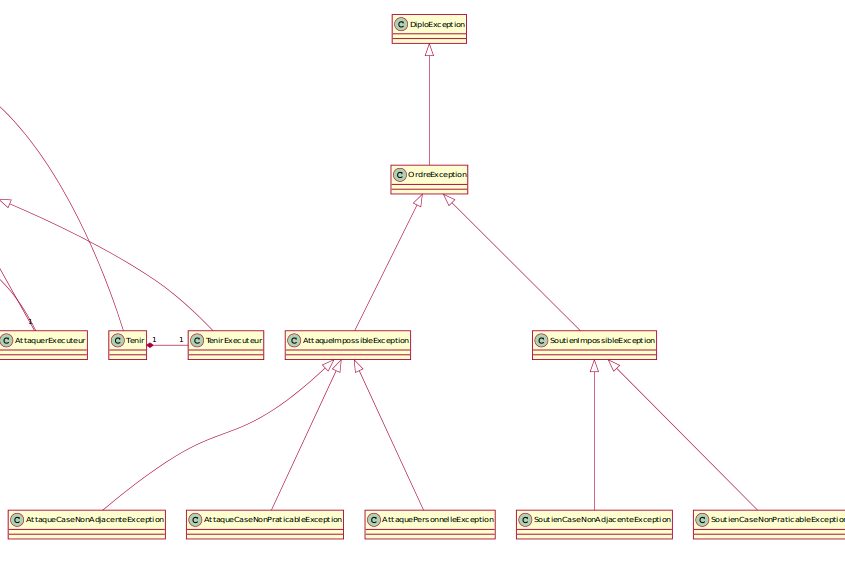
\includegraphics[scale=0.5]{images/DCP3.png}
		\caption{Les exceptions}
	\end{figure}
\newpage
\section{Diagramme de packages}
\subsection{Première partie}
	\vspace{10mm}
	\begin{figure}[!h]
		\centering
		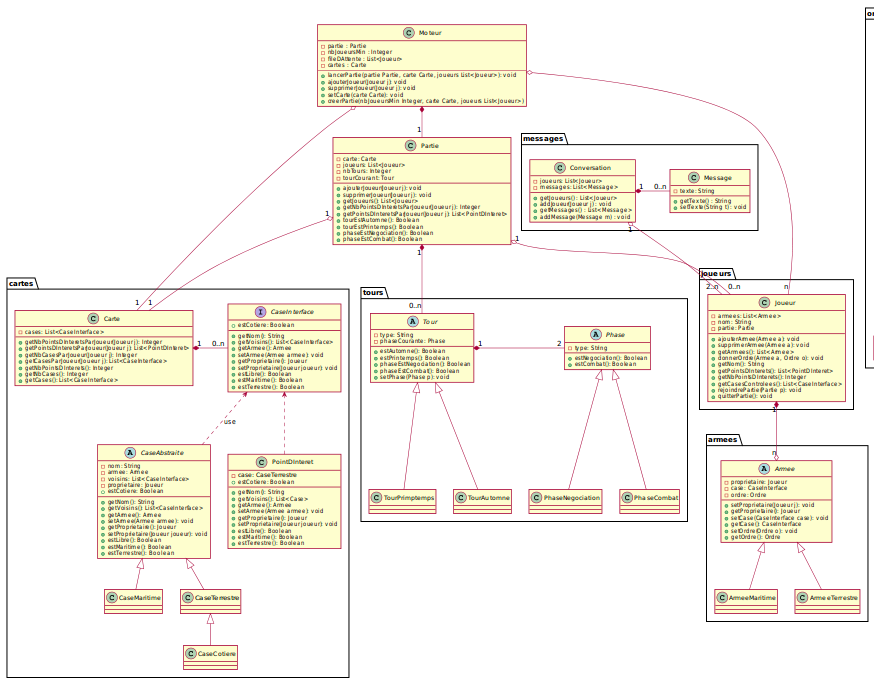
\includegraphics[angle=90,width=150mm]{images/DP1.png}
		\caption{Première partie}
	\end{figure}
\newpage
\subsection{Deuxième partie}
	\vspace{10mm}
	\begin{figure}[!h]
		\centering
		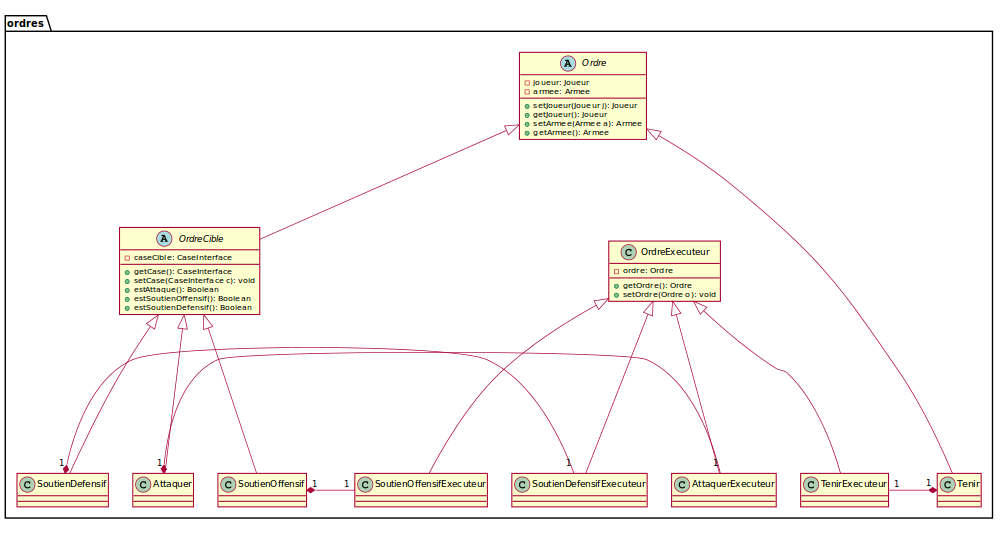
\includegraphics[scale=0.4]{images/DP2.png}
		\caption{Le package Ordres}
	\end{figure}

\subsection{Troisième partie}
	\vspace{10mm}
	\begin{figure}[!h]
		\centering
		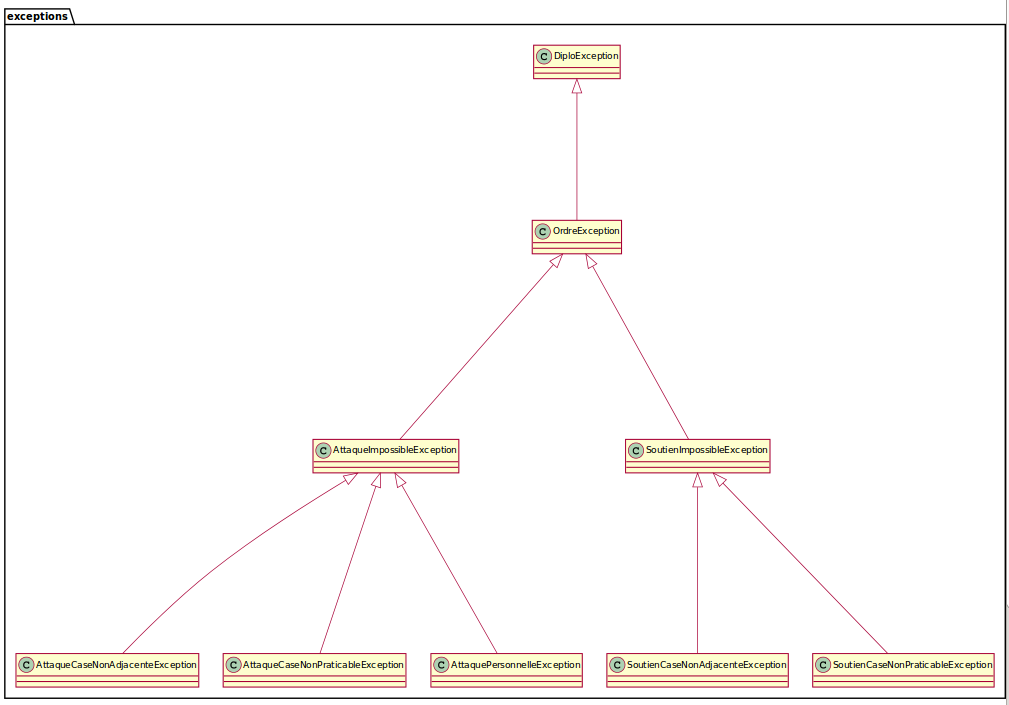
\includegraphics[scale=0.4]{images/DP3.png}
		\caption{Le package Exceptions}
	\end{figure}

\newpage
\section{Diagramme de séquence système}
\subsection{Créer une partie}
	\vspace{10mm}
	\begin{figure}[!h]
		\centering
		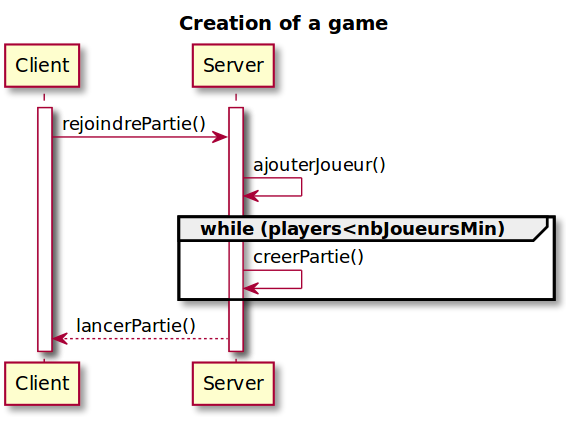
\includegraphics[scale=0.5]{images/DSSCreate.png}
		\caption{Créer une partie}
	\end{figure}


\subsection{Jouer son tour}
	\vspace{10mm}
	\begin{figure}[!h]
		\centering
		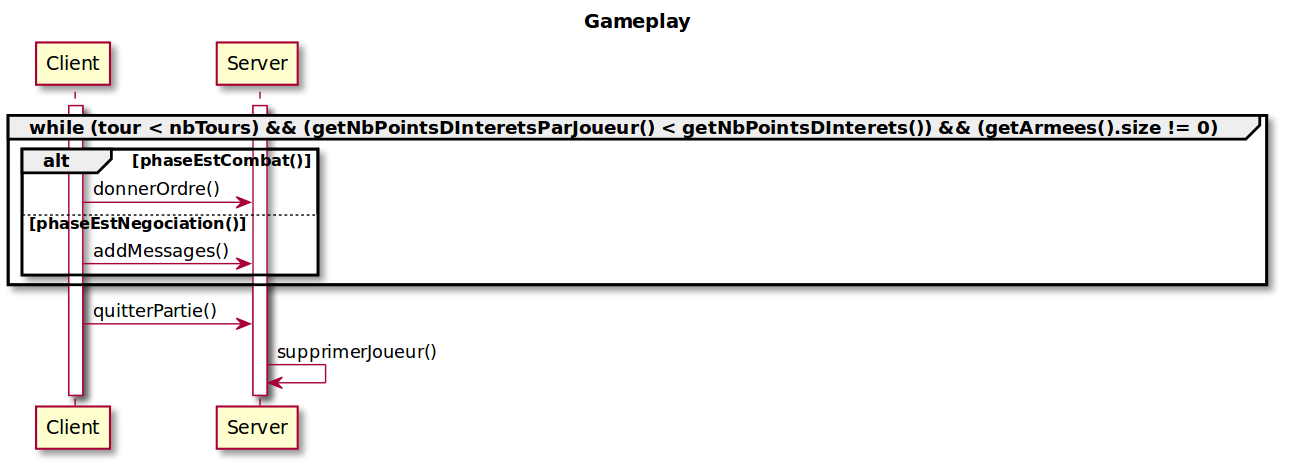
\includegraphics[scale=0.3]{images/DSSGameplay.png}
		\caption{Jouer son tour}
	\end{figure}
	\vspace{70mm}

\section{Sources du DCP et du diagramme de package}
\begin{itemize}
	\item DCP : \url{http://goo.gl/7uLQP4}
	\item Diagramme de Package : \url{http://goo.gl/LsiHrs}
\end{itemize}